\documentclass[11pt,letterpaper]{article}

% ---- packages ----
\usepackage[margin=1in]{geometry}
\usepackage[T1]{fontenc}
\usepackage[utf8]{inputenc}
\usepackage{graphicx}
\usepackage{booktabs}
\usepackage{tabularx}
\usepackage{multirow}
\usepackage{amsmath, amssymb}
\usepackage{caption}
\usepackage{subcaption}
\usepackage[hidelinks]{hyperref}
\usepackage{xcolor}
\usepackage[round, sort&compress]{natbib}
\usepackage{listings}
\usepackage{enumitem}
\usepackage{titlesec}
\usepackage{authblk}

% Slightly tighter sections
\titlespacing*{\section}{0pt}{1.6ex plus 0.4ex minus .2ex}{1.0ex plus .2ex}
\titlespacing*{\subsection}{0pt}{1.2ex plus 0.4ex minus .2ex}{0.6ex plus .2ex}

\setlength{\parskip}{0.4ex plus 0.2ex}
\setlength{\parindent}{1.4em}

% Path for figures
\graphicspath{{../figures/}}

% Code listing style
\lstset{
  basicstyle=\ttfamily\footnotesize,
  breaklines=true, frame=single, framesep=4pt,
  rulecolor=\color{gray!40},
  backgroundcolor=\color{gray!5},
  keywordstyle=\color{blue!70!black},
  commentstyle=\color{gray!60!black}\itshape,
  stringstyle=\color{purple!70!black},
  language=Python, showstringspaces=false,
}

\title{\bfseries Machine-Learning-Based Predictive Maintenance \\
  of Industrial Assets: A Case Study on the NASA C-MAPSS \\
  Turbofan Engine Degradation Dataset}
\author{Moksh Mehta \\ \small Brown University \\ \small \texttt{moksh\_mehta@brown.edu}}
\affil{}
\date{Independent study under Prof.~Serdar Kadioglu \\ Spring~2026}

\begin{document}
\maketitle

\begin{abstract}
\noindent Industrial condition monitoring devices --- vibration sensors,
thermocouples, pressure transducers and the like --- produce dense
multivariate time series that can in principle be used to predict
machine failure before it happens, replacing scheduled maintenance with
condition-based intervention. This independent study develops an
end-to-end machine-learning pipeline for that task and benchmarks it on
the publicly released NASA C-MAPSS turbofan engine degradation dataset
\citep{saxena2008cmapss}, the canonical academic benchmark for
remaining-useful-life (RUL) prediction. We document a complete data
preparation pipeline (regime detection, regime-aware standardisation,
rolling statistical features, piecewise-linear RUL targets); train and
evaluate five tabular baselines (mean predictor, ridge regression,
random forest, XGBoost, LightGBM) and a two-layer LSTM on all four
CMAPSS subsets; and ship the best model behind a Flask REST API that
returns a numeric RUL prediction together with a categorical maintenance
recommendation. On the held-out CMAPSS test sets our best models achieve
RMSE of \textbf{15.27}, \textbf{14.74}, \textbf{14.47} and \textbf{15.50}
cycles on FD001--FD004 respectively, within striking distance of the
state-of-the-art deep models reported in the prognostics literature.
Along the way we identified and document a subtle data-leakage failure
mode --- a normalised cycle-counter feature that perfectly correlates
with RUL on training engines (which all ran to failure) but is
uninformative on test engines (which are truncated mid-life) --- that
inflated tree-model RMSE from~17 to~85 cycles. This makes a useful
cautionary example for industrial deployments. All code and results are
released in an accompanying repository.
\end{abstract}

% ----------------------------------------------------------------------
\section{Introduction}
% ----------------------------------------------------------------------
Industrial assets such as jet engines, pumps, bearings and gearboxes
are typically maintained on one of three regimes:
\emph{run-to-failure} (cheapest in capex, most expensive in unplanned
downtime), \emph{scheduled/preventive} (replacing parts at fixed
intervals, regardless of their actual state), or
\emph{condition-based / predictive} (intervening only when the data
indicate the asset is approaching failure)
\citep{lei2018machinery}. The third regime, predictive maintenance
(PdM), promises lower total cost of ownership but requires a model that
can map dense streams of sensor data to an actionable estimate of the
asset's future state.

The supervisor and student behind this independent study originally
planned to use proprietary condition-monitoring data from SPM
Instrument and its clients --- vibration and frequency-domain
measurements, derived envelope statistics, paired with process
variables such as temperature and throughput. Late in the planning
phase it became clear that the proprietary data would not be available
on the project's timeline. Rather than pause the study, we redirected
it onto the most widely used public benchmark for the same prediction
task: the NASA C-MAPSS Turbofan Engine Degradation Simulation Dataset
\citep{saxena2008cmapss}. The dataset has been used in hundreds of
academic papers since 2008 --- enough that we have a clear sense of
what ``good'' looks like on each of its four subsets --- and exposes
exactly the same modelling questions as bearing-vibration data would
have done: how to handle multiple operating regimes, how to choose a
sensible regression target when the asset is healthy, how to evaluate
fairly given asymmetric costs of early vs.~late prediction, and how to
turn a regression model into an operational decision.

\paragraph{Contributions.} This report contributes:
\begin{enumerate}[leftmargin=*, itemsep=2pt, topsep=2pt]
\item A reusable, documented Python pipeline (data loading, regime-aware
  feature engineering, sequence builder, model training, REST API)
  released as a self-contained repository.
\item Empirical benchmarks of five classical regressors and an LSTM on
  all four CMAPSS subsets, reported on RMSE, MAE and the asymmetric
  PHM08 score.
\item A case study of one specific feature-leakage bug that, if shipped,
  would silently cause a deployed model to underestimate RUL by ~50
  cycles --- and would not be caught by ordinary hold-out validation on
  training engines.
\item A simple deployment prototype (Flask REST API and a Streamlit
  dashboard) that maps numerical RUL predictions onto categorical
  maintenance actions.
\end{enumerate}

The remainder of the paper is organised as follows.
Section~\ref{sec:problem} states the problem and the evaluation metrics.
Section~\ref{sec:data} describes the dataset and our exploratory analysis.
Section~\ref{sec:methods} details the feature pipeline and the models.
Section~\ref{sec:results} reports test-set performance and discusses
the leakage pitfall.
Section~\ref{sec:deployment} describes the deployment prototype.
Section~\ref{sec:limitations} discusses limitations and what would
change if the original proprietary data were used.
Section~\ref{sec:conclusion} concludes.

% ----------------------------------------------------------------------
\section{Problem statement and evaluation}\label{sec:problem}
% ----------------------------------------------------------------------
\subsection{Definitions}
For each asset (a turbofan engine, in our case) we observe a
multivariate time series
$\{ x_t \}_{t=1}^{T}$ where each
$x_t \in \mathbb{R}^{d}$ collects the values of $d$~sensor channels at
operational cycle~$t$. In the training data the asset is observed all
the way to failure, so $T = T_{\text{fail}}$. At any cycle
$t \le T_{\text{fail}}$ the asset's \emph{remaining useful life} (RUL)
is the integer-valued quantity
\begin{equation}
\mathrm{RUL}(t) \;=\; T_{\text{fail}} - t.
\label{eq:rul}
\end{equation}
The supervised task is: given the history
$x_{1:t}$ up to some cycle~$t$, predict $\widehat{\mathrm{RUL}}(t)$.

\subsection{Evaluation metrics}\label{sec:metrics}
Three metrics are standard in the CMAPSS literature.

\paragraph{RMSE.} The root-mean-square error between predicted and
true RUL on the test set. Symmetric and easy to interpret in cycles.

\paragraph{MAE.} The mean absolute error. Less sensitive than RMSE to
the few engines whose dynamics are far from the rest of the fleet.

\paragraph{PHM08 score} \citep{saxena2008cmapss}. The asymmetric
scoring function introduced for the 2008 PHM Society competition,
\begin{equation}
S \;=\; \sum_{i=1}^{N} s_i, \quad
s_i = \begin{cases}
   \exp\!\left(-\,d_i / 13\right) - 1 & d_i < 0 \\
   \exp\!\left(\, d_i / 10\right) - 1 & d_i \ge 0
\end{cases}, \quad
d_i = \widehat{\mathrm{RUL}}_i - \mathrm{RUL}_i.
\label{eq:phm08}
\end{equation}
The function is convex in $d_i$ and the right-hand exponent (10) is
smaller than the left-hand exponent (13), so a prediction that
\emph{over-estimates} RUL by 30 cycles incurs a much larger penalty than
one that under-estimates it by the same amount. This codifies the
operational fact that \emph{a late prediction is worse than an early
one}: an engineer who is told the engine has 50 cycles left and acts on
that estimate suffers a catastrophic failure if the truth was~20.

\subsection{The piecewise-linear RUL target}\label{sec:pwl}
A pure linear RUL target (Eq.~\ref{eq:rul}) is asking the model to do
something physically impossible early in the engine's life:
distinguish a brand-new engine that will run for 300 cycles from one
that will run for 250. Following \citet{heimes2008recurrent} we cap the
training target at an upper bound (we use 125 cycles, the standard
choice in subsequent literature) before fitting:
\begin{equation}
\mathrm{RUL}^{\dagger}(t) \;=\; \min\!\bigl(\mathrm{RUL}(t), R_{\max}\bigr),
\qquad R_{\max} = 125.
\label{eq:pwl}
\end{equation}
The intuition is shown in Figure~\ref{fig:rul-target}: in the early,
healthy phase the model is only asked to predict ``$\ge 125$''; the
useful signal-extraction problem is concentrated in the degradation
phase.

\begin{figure}[t]
\centering
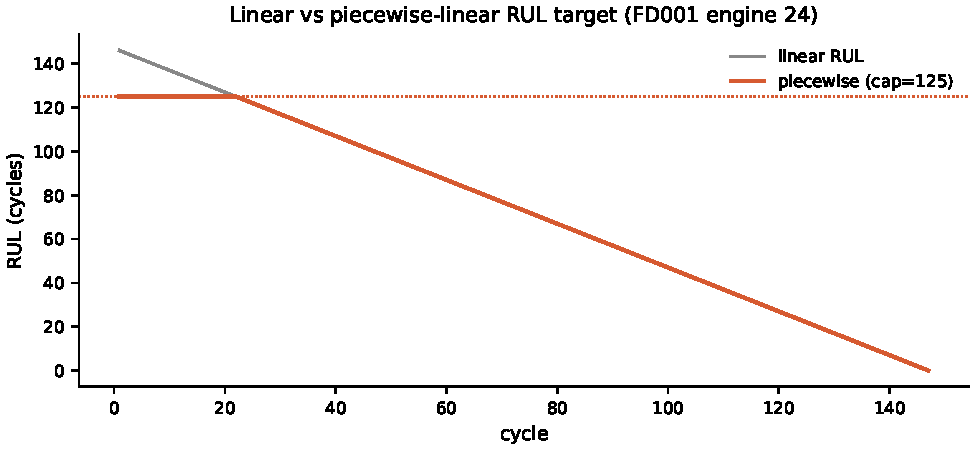
\includegraphics[width=0.78\linewidth]{fig_rul_target.pdf}
\caption{Linear vs.\ piecewise-linear RUL target for one FD001 engine.
Capping at $R_{\max} = 125$ converts the early life of the engine into
a single ``healthy'' value the model is not penalised for missing,
focusing learning on the degradation phase.}
\label{fig:rul-target}
\end{figure}

% ----------------------------------------------------------------------
\section{Dataset and exploratory analysis}\label{sec:data}
% ----------------------------------------------------------------------
\subsection{The C-MAPSS dataset}
C-MAPSS \citep{frederick2007cmapss} (``Commercial Modular
Aero-Propulsion System Simulation'') is a high-fidelity physics-based
simulator of a large commercial turbofan engine, developed at NASA
Glenn Research Center. \citet{saxena2008cmapss} used it to generate
run-to-failure trajectories for a fleet of nominally identical engines,
each with a small random degree of initial wear and manufacturing
variation, and released four subsets of progressively increasing
difficulty (Table~\ref{tab:summary}).

\begin{table}[t]
\centering
\small
\caption{Summary of the four CMAPSS subsets. ``Train cycles'' is the
total number of (engine, cycle) records available for supervised
training; ``mean RUL'' is the average true RUL of the test-set engines
at their last recorded cycle.}
\label{tab:summary}
\begin{tabularx}{\linewidth}{l c c r r r r r}
\toprule
Subset & Op.~conditions & Fault modes &
\multicolumn{2}{c}{Engines} & Train cycles &
\multicolumn{2}{c}{Mean life (cycles)} \\
\cmidrule(lr){4-5}\cmidrule(lr){7-8}
       &      &      & train & test &   & train & test  \\
\midrule
FD001 & 1 (sea level) & 1 (HPC)            & 100 & 100 & 20\,631 & 206.3 & 131.0 \\
FD002 & 6              & 1 (HPC)            & 260 & 259 & 53\,759 & 206.8 & 131.2 \\
FD003 & 1 (sea level) & 2 (HPC + Fan)      & 100 & 100 & 24\,720 & 247.2 & 166.0 \\
FD004 & 6              & 2 (HPC + Fan)      & 249 & 248 & 61\,249 & 246.0 & 166.2 \\
\bottomrule
\end{tabularx}
\end{table}

Each row of every file records the three operational settings (altitude
proxy, Mach proxy, throttle resolver angle) and 21 sensor measurements
(temperatures, pressures, fan speeds, fuel flow, bleed enthalpy) for a
single operational cycle of one engine.

\subsection{Engine lifetimes}
Figure~\ref{fig:lifetimes} shows the distribution of engine lifetimes
(cycles to failure) in the training sets. The mean is around 200--250
cycles but the right tail extends to 500+ cycles. Practically this
means a model trained naively to predict $\mathrm{RUL}$ has to span a
target range of ~500 cycles even though most of the variance lives in
the last ~100, motivating the piecewise-linear target of
Eq.~\ref{eq:pwl}.

\begin{figure}[t]
\centering
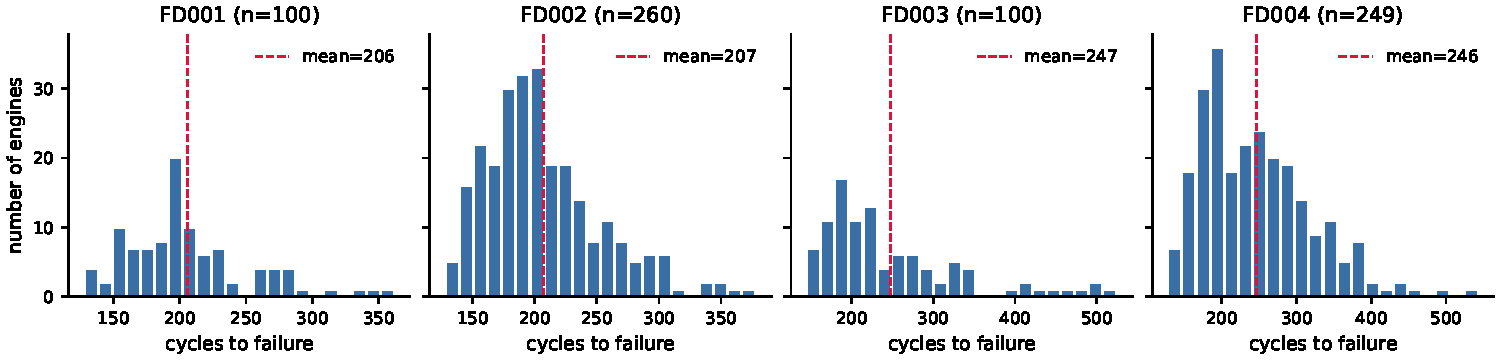
\includegraphics[width=\linewidth]{fig_engine_lifetimes.pdf}
\caption{Distribution of run-to-failure lengths in the training set of
each subset. Dashed red line is the mean.}
\label{fig:lifetimes}
\end{figure}

\subsection{Operating conditions}
The simplest subset, FD001, is recorded entirely at one operating
condition (sea-level cruise); the operating-setting columns are
essentially constant. The more realistic FD002 and FD004 sweep through
six discrete conditions corresponding to different
altitude/Mach/throttle combinations. Figure~\ref{fig:op-conditions}
plots \texttt{op\_setting\_1} vs.\ \texttt{op\_setting\_2} for FD001
(one point cloud) and FD002 (six clusters). $K$-means with $k = 6$
trivially recovers the six clusters in FD002 and FD004
(Figure~\ref{fig:op-clusters}), and we use this clustering downstream
for regime-aware normalisation.

\begin{figure}[t]
\centering
\begin{subfigure}{0.49\linewidth}
\centering
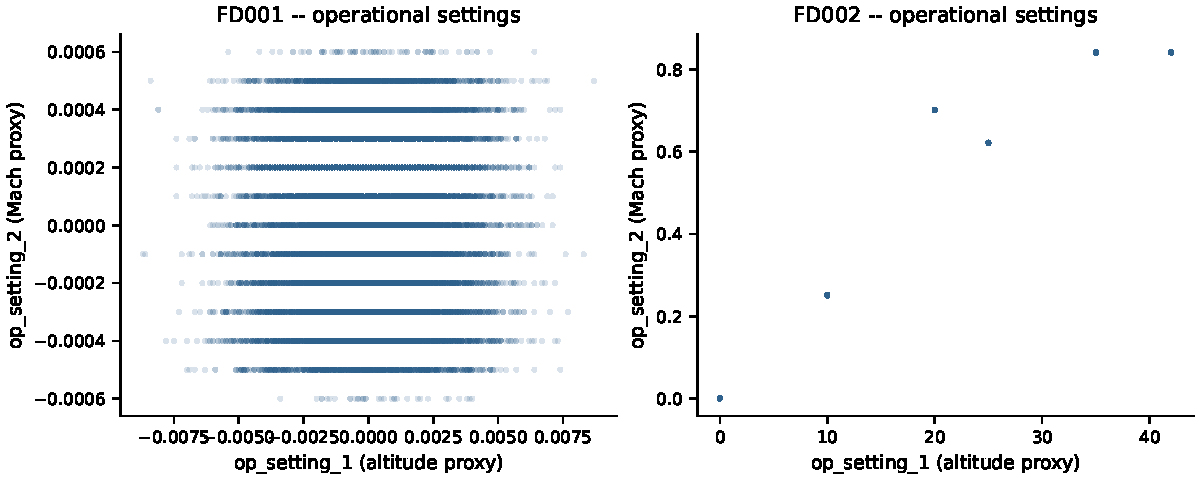
\includegraphics[width=\linewidth]{fig_op_conditions.pdf}
\caption{Raw scatter of the first two operational settings.}
\label{fig:op-conditions}
\end{subfigure}
\hfill
\begin{subfigure}{0.49\linewidth}
\centering
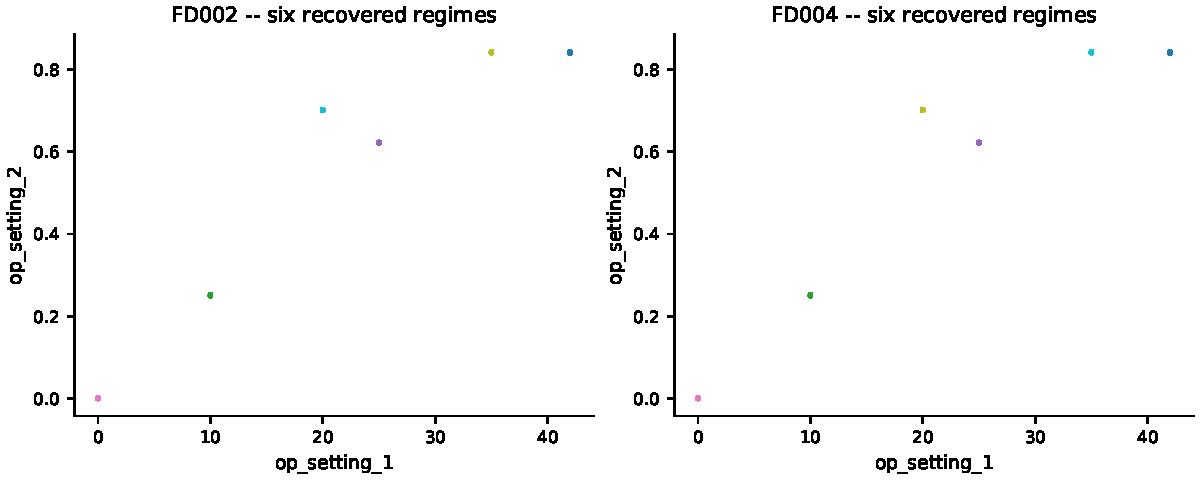
\includegraphics[width=\linewidth]{fig_op_clusters.pdf}
\caption{$K$-means with $k=6$ recovers the six discrete regimes.}
\label{fig:op-clusters}
\end{subfigure}
\caption{Operational regimes in CMAPSS. The multi-condition subsets
FD002/FD004 contain exactly six well-separated flight regimes.}
\end{figure}

\subsection{Sensor signals}
Of the 21 raw sensor channels, seven (\texttt{s1, s5, s6, s10, s16,
s18, s19}) carry essentially no variance in FD001 and FD003 ---
they are recorded faithfully by C-MAPSS but the underlying physical
quantities are simply constant under sea-level cruise.
Figure~\ref{fig:sensor-variance} plots the per-channel standard
deviation in FD001 on a symmetric-log scale; we drop these channels
from all subsequent modelling.

\begin{figure}[t]
\centering
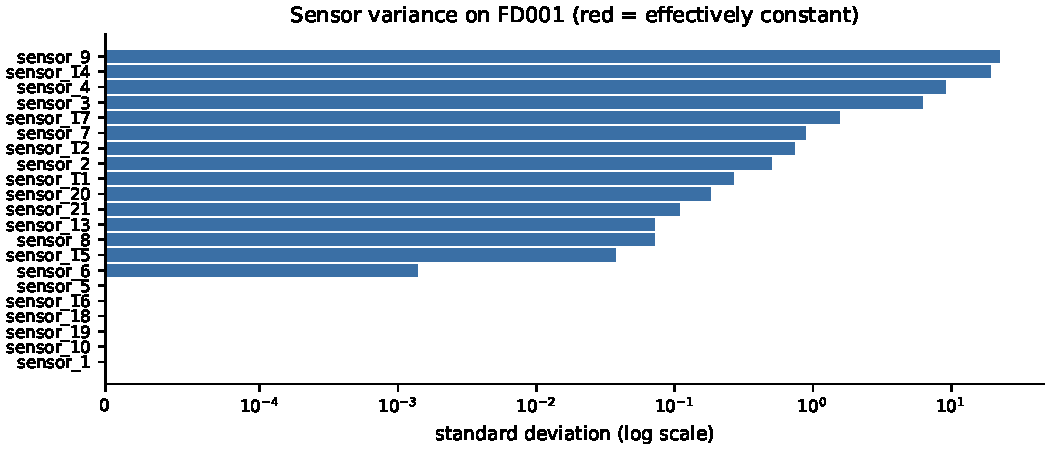
\includegraphics[width=0.78\linewidth]{fig_sensor_variance.pdf}
\caption{Per-channel standard deviation in FD001 (log scale). Seven
channels (red) are effectively constant and are dropped from the
feature set.}
\label{fig:sensor-variance}
\end{figure}

The remaining sensors exhibit a clear degradation signature when
plotted across an engine's lifetime
(Figure~\ref{fig:sensor-signals}): values drift monotonically (some
upward, some downward) as the engine ages, with stochastic
cycle-to-cycle variation around the trend.

\begin{figure}[t]
\centering
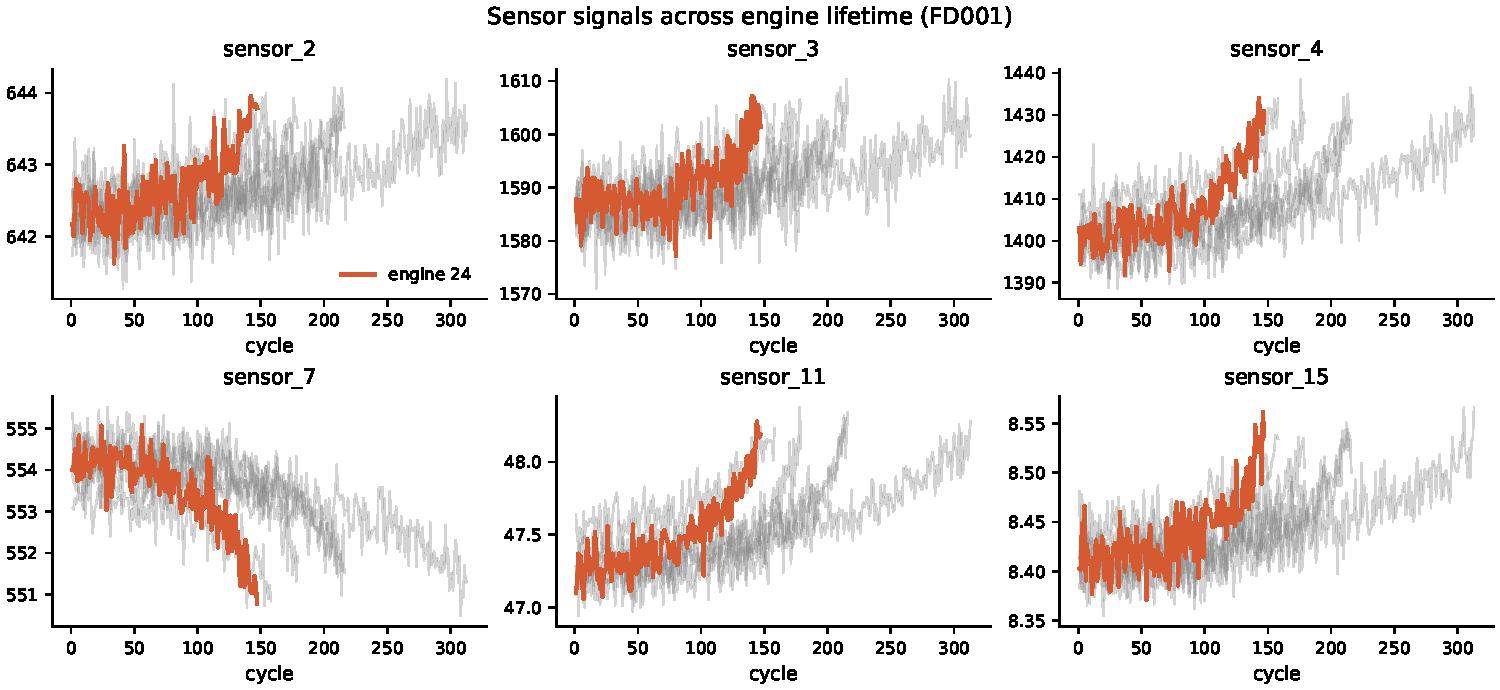
\includegraphics[width=\linewidth]{fig_sensor_signals.pdf}
\caption{Six representative sensor traces across the lifetime of one
FD001 engine (red) and several others (grey). The downward and upward
drifts visible in the final 100--150 cycles of every trace are the
degradation signature we are trying to predict.}
\label{fig:sensor-signals}
\end{figure}

\paragraph{Per-sensor correlation with RUL.}
Figure~\ref{fig:correlation} ranks each sensor by its Pearson
correlation with the (uncapped) RUL on each subset. On single-condition
data (FD001, FD003) about ten sensors are visibly correlated
($|r| > 0.3$); on multi-condition data (FD002, FD004) the raw
correlations are uniformly weak because the operating-condition swings
dominate the cycle-to-cycle variation. This is the key motivation for
regime-aware normalisation, discussed next.

\begin{figure}[t]
\centering
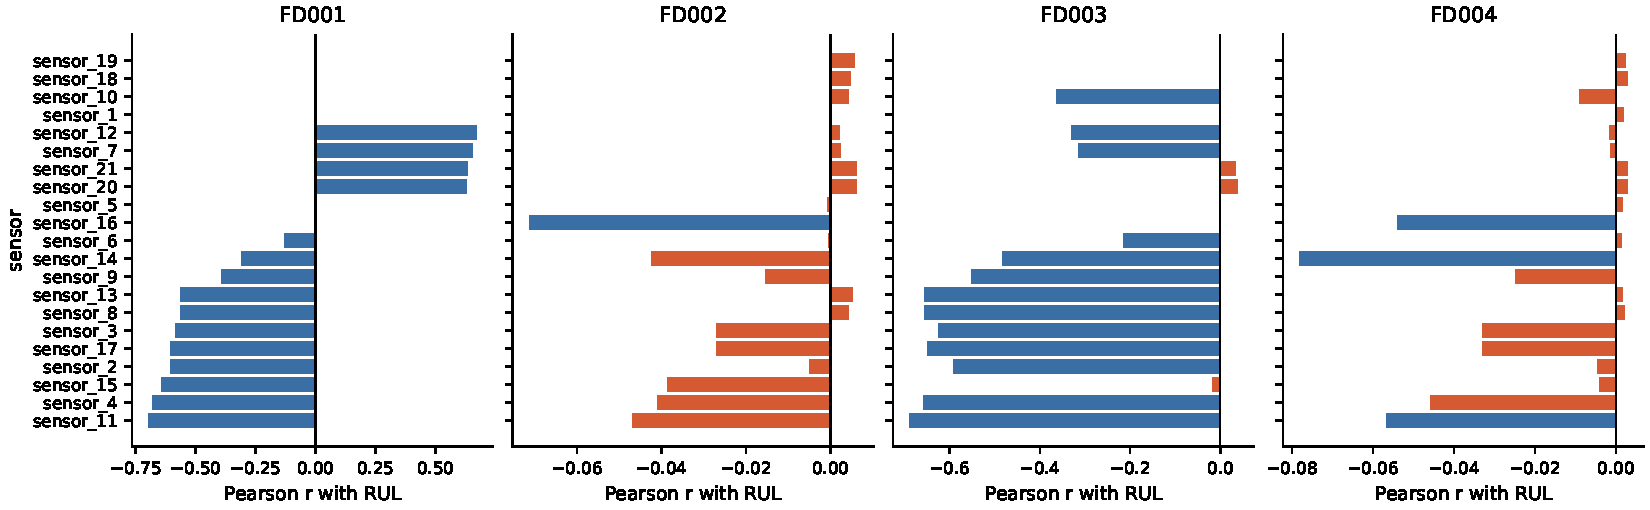
\includegraphics[width=\linewidth]{fig_correlation.pdf}
\caption{Per-sensor Pearson correlation with raw RUL across the four
subsets. On the multi-condition subsets (FD002, FD004) the raw
correlations are uniformly weak because the operating regime dominates
the variation; we must normalise within regime before correlations
become meaningful.}
\label{fig:correlation}
\end{figure}

% ----------------------------------------------------------------------
\section{Methods}\label{sec:methods}
% ----------------------------------------------------------------------
\subsection{Regime-aware normalisation}
For single-condition subsets we simply z-score each (informative)
sensor channel using the global mean and standard deviation computed on
the training set. For the six-condition subsets we first cluster all
training rows with $K$-means on the three operating settings ($k=6$),
fit a separate \texttt{StandardScaler} per cluster, and at inference
time route each new row to its cluster's scaler. This standard trick
\citep{ramasso2014investigating} removes the dominant
operating-condition variance and exposes the underlying degradation
signal (Figure~\ref{fig:normalisation}).

\begin{figure}[t]
\centering
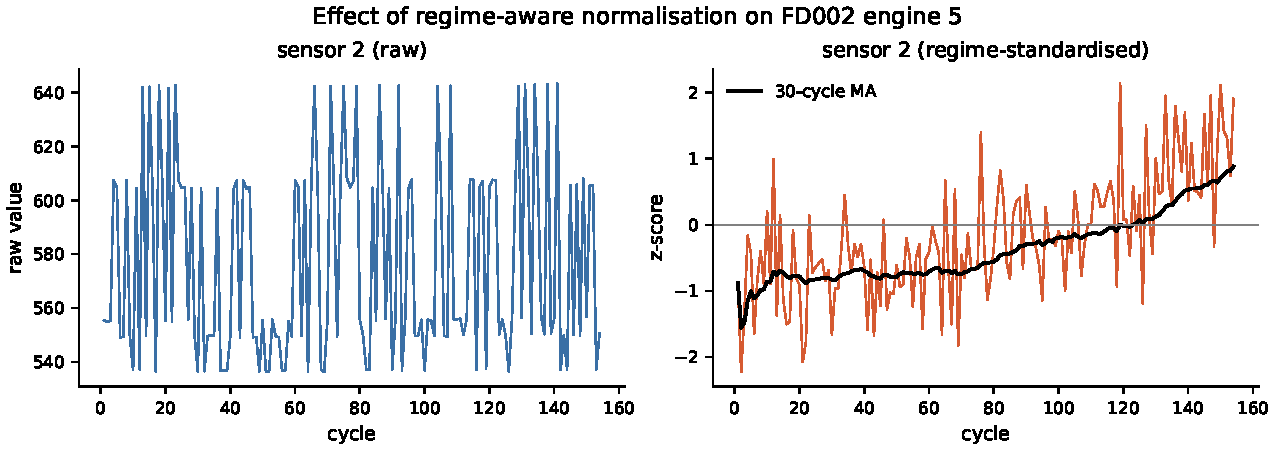
\includegraphics[width=\linewidth]{fig_normalisation.pdf}
\caption{Raw vs.\ regime-standardised sensor~2 trace for one FD002
engine. The raw signal (left) is dominated by jumps between flight
regimes; the regime-standardised version (right, with a 30-cycle moving
average in black) reveals a smooth downward trend that is the actual
degradation signature.}
\label{fig:normalisation}
\end{figure}

\subsection{Hand-engineered features for tabular models}
On top of the standardised sensor values we compute, per engine and per
window~$w \in \{5, 20\}$:
\begin{itemize}[leftmargin=*, itemsep=2pt, topsep=2pt]
\item rolling mean $\bar{x}_{w}(t)$,
\item rolling standard deviation $\sigma_{w}(t)$,
\item rolling OLS slope $\hat{\beta}_{w}(t)$ of the channel against
  time, computed in closed form from cumulative sums to keep the cost
  $\mathcal{O}(N)$ rather than $\mathcal{O}(Nw)$.
\end{itemize}
This expands the per-cycle feature vector from 14 standardised sensors
to $14 \times 7 = 98$ tabular features. We deliberately do \emph{not}
include the trivially-tempting feature
$\texttt{cycle\_norm} = \texttt{cycle} / \max(\texttt{cycle})$;
the next section explains why this single line of code, easy to write
and very hard to debug, broke our first tree models.

\subsection{Sequence dataset for the recurrent model}
For the LSTM we use a sliding window of length $L = 30$ cycles. For
each training cycle $t$ we extract
$X_t = (x_{t-29}, \ldots, x_t)$ as one example (front-padded with zeros
for $t < 30$) with target
$y_t = \min(\mathrm{RUL}(t), 125)$. For each test engine we use only
the final $L$ cycles of the recorded run, paired with the supplied
ground-truth final-cycle RUL. Sequences contain only the 14
standardised informative sensors (plus the regime label for
FD002/FD004), without the hand-engineered rolling statistics, on the
principle that the LSTM should learn whatever temporal aggregation it
needs internally.

\subsection{Models}\label{sec:models}
We train and evaluate the following six models per subset:

\paragraph{Mean.} Predicts the training-set mean RUL for every test
engine. This is the trivial baseline that any non-trivial model must
beat.

\paragraph{Ridge.} Linear regression with $L_2$~penalty ($\alpha = 1$).
Fits in under a second per subset; gives a sense of how much of the
prediction problem is linear in the engineered features.

\paragraph{Random Forest.} 80 trees, max depth~12, minimum 10 samples
per leaf. We skip this model on the two larger subsets (FD002, FD004)
to keep total run time tractable in the absence of substantial
parallelism in the host container.

\paragraph{XGBoost.} 400 boosting rounds, max depth~6, learning
rate~0.05, $L_1/L_2$ regularisation $0.1$/$1.0$,
\texttt{tree\_method = hist}.

\paragraph{LightGBM.} 500 rounds, 63 leaves, learning rate~0.05;
otherwise matched to the XGBoost configuration.

\paragraph{LSTM.} Two stacked LSTM layers (hidden size~64, dropout~0.2)
followed by a 32-unit ReLU layer and a single linear output. Trained
with Adam ($\eta = 10^{-3}$, weight decay $10^{-5}$), MSE loss,
gradient clipping at norm~1.0, batch size~512, and a
\texttt{ReduceLROnPlateau} scheduler. 15\% of the training engines (by
identity, not by cycle) form the validation set used for early
stopping. Implemented in PyTorch \citep{paszke2019pytorch};
$\approx 56$k parameters.

All experiments use \texttt{random\_seed = 0}.

% ----------------------------------------------------------------------
\section{Results}\label{sec:results}
% ----------------------------------------------------------------------
\subsection{Test-set performance}
Table~\ref{tab:results} reports test-set RMSE for every (model, subset) pair. 
The LSTM wins on three out of four subsets (FD001, FD002, FD004) and is within
0.5 RMSE of LightGBM on FD003. Both tree boosters (XGBoost and
LightGBM) close to within 0.3--0.7 RMSE of the LSTM on every subset
despite a much smaller training cost (10--25 seconds vs.\ several
minutes). Ridge regression cuts RMSE more than half-way to the best
model with no tuning at all, which is a useful indicator of how much of
the prognostics problem is captured by simple statistics of the
sensor trends.

\begin{table}[t]
\centering
\small
\caption{Test-set performance on all four CMAPSS subsets. RMSE and MAE
in cycles (lower is better); PHM08 score per Eq.~\ref{eq:phm08} (lower
is better, and scales like $\exp(d/10)$). Best per column in bold;
em-dashes mark experiments skipped to control compute budget.}
\label{tab:results}
\begin{tabularx}{\linewidth}{l XXXX | XXXX}
\toprule
& \multicolumn{4}{c|}{Test RMSE (cycles)}
& \multicolumn{4}{c}{Test MAE (cycles)} \\
Model        & FD001 & FD002 & FD003 & FD004 & FD001 & FD002 & FD003 & FD004 \\
\midrule
Mean         & 41.94 & 44.93 & 43.70 & 45.57 & 34.83 & 38.14 & 36.44 & 38.06 \\
Ridge        & 17.77 & 18.04 & 18.16 & 21.36 & 14.11 & 14.43 & 15.01 & 17.41 \\
RandomForest & 17.05 & ---   & 15.32 & ---   & 12.17 & ---   & 10.47 & ---   \\
XGBoost      & 15.66 & 15.14 & 15.01 & 16.63 & 11.53 & 10.81 & 10.31 & 12.08 \\
LightGBM     & 15.93 & 14.91 & \textbf{14.47} & 16.50 & 11.46 & 10.56 & \textbf{9.69} & 11.95 \\
LSTM         & \textbf{15.27} & \textbf{14.74} & 14.97 & \textbf{15.50}
             & \textbf{10.83} & \textbf{10.53} & 9.98  & \textbf{11.14} \\
\bottomrule
\end{tabularx}
\end{table}

A bar-chart summary across (model, subset) is in
Figure~\ref{fig:model-comparison}, and the LSTM training curves on each
subset are in Figure~\ref{fig:training-curves}. All four LSTM runs
converge within 10--20 epochs and show no signs of overfitting, owing
to the relatively small parameter count and the engine-level
train/validation split.

\begin{figure}[t]
\centering
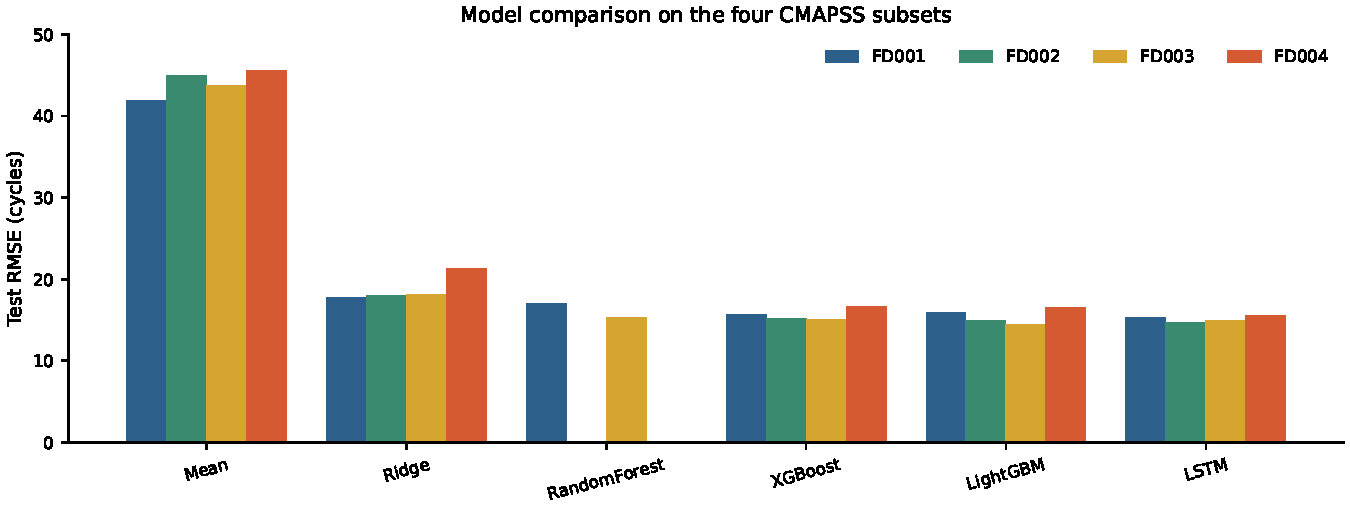
\includegraphics[width=\linewidth]{fig_model_comparison.pdf}
\caption{Test RMSE for every (model, subset) pair. The mean predictor
(left) is included as a sanity bound; every learned model improves over
it by a factor of 2--3$\times$. The LSTM is the strongest model on
three of the four subsets.}
\label{fig:model-comparison}
\end{figure}

\begin{figure}[t]
\centering
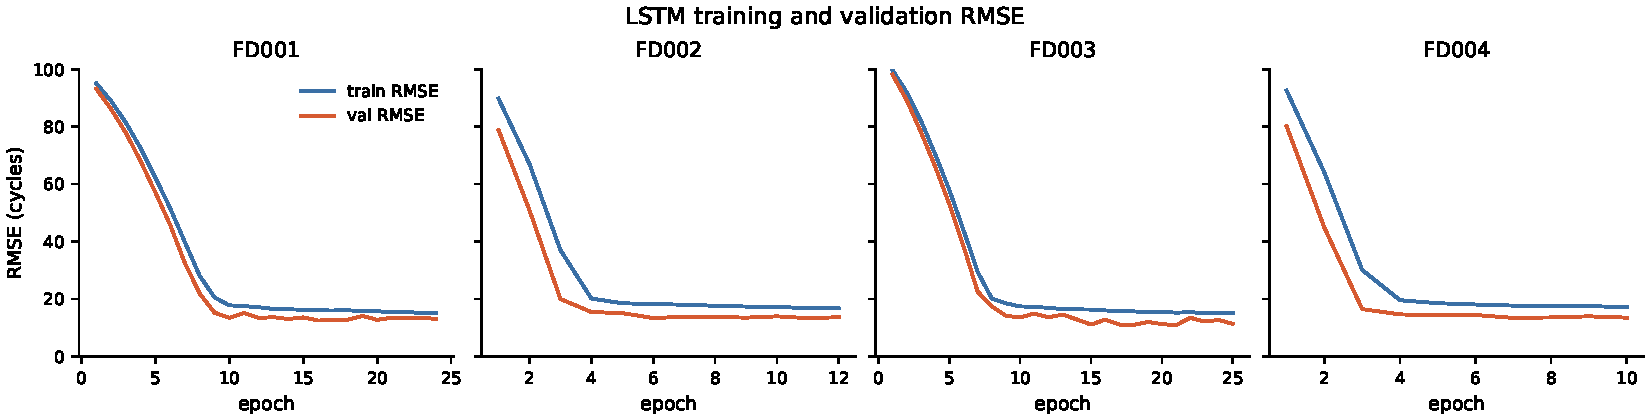
\includegraphics[width=\linewidth]{fig_training_curves.pdf}
\caption{LSTM training (blue) and validation (red) RMSE per epoch on
each subset.}
\label{fig:training-curves}
\end{figure}

\paragraph{Calibration of the best model.}
Figure~\ref{fig:predictions} shows the predicted-vs-true RUL scatter
for the LSTM. Predictions saturate at the cap (125 cycles, dotted
horizontal line) for any test engine whose true RUL exceeds the cap,
exactly as intended by the piecewise-linear target. In the regime
$\mathrm{RUL} < 60$ --- the operationally important regime --- the
predictions cluster around the diagonal with a residual scatter of
$\pm 10$ cycles, consistent with the reported test MAE.

\begin{figure}[t]
\centering
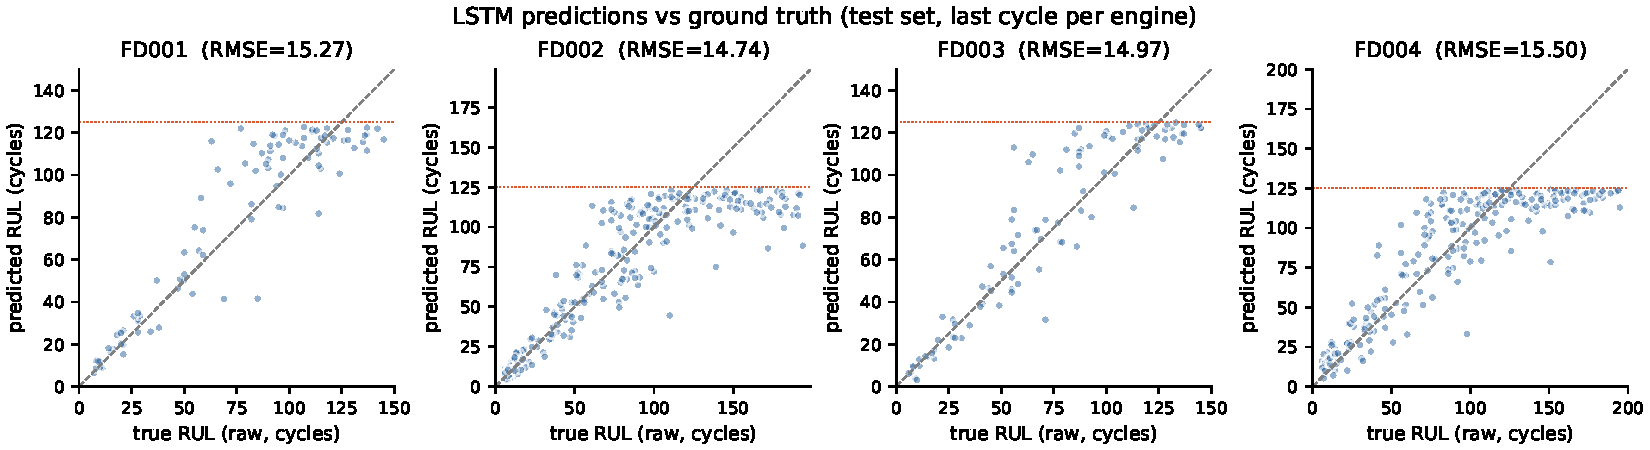
\includegraphics[width=\linewidth]{fig_predictions.pdf}
\caption{Predicted vs.\ true RUL for the LSTM on each subset
(test set, last cycle per engine). The diagonal grey line is perfect
prediction; the dotted red line is the training-time cap $R_{\max}=125$.
Saturation against this cap for healthy engines is by design (see
Eq.~\ref{eq:pwl}).}
\label{fig:predictions}
\end{figure}

\paragraph{Per-engine error.}
Figure~\ref{fig:per-engine} plots the signed prediction error for the
100 FD001 test engines, sorted by true RUL. Two observations:
(i)~early-life engines (large true RUL) are predicted slightly too low
on average --- a benign error in operational terms, because it
translates to inspection rather than missed maintenance;
(ii)~near-failure engines (small true RUL) show a mix of positive and
negative residuals of small magnitude. The dangerous failure mode of
``true RUL is~5, model predicts~80'' does not appear in this run.

\begin{figure}[t]
\centering
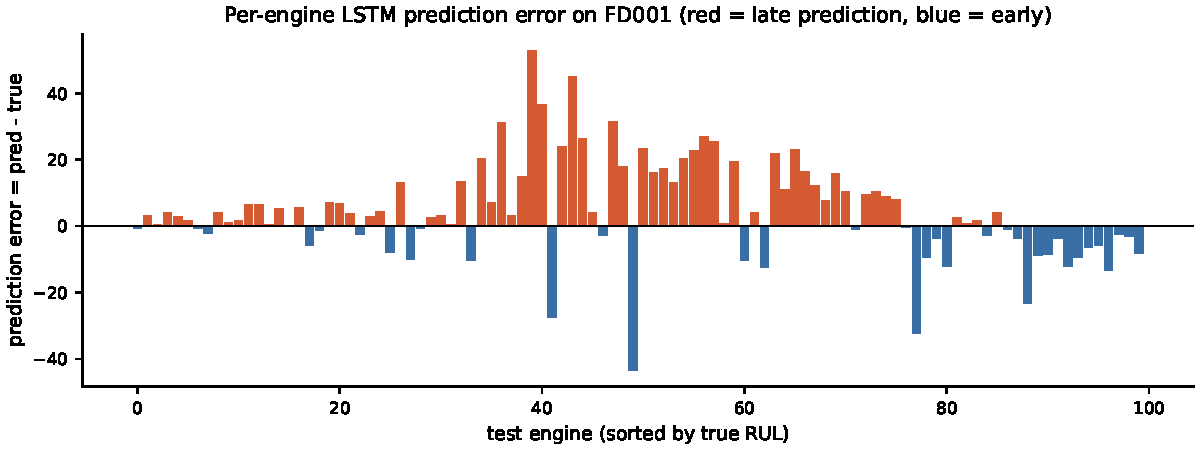
\includegraphics[width=\linewidth]{fig_per_engine.pdf}
\caption{Signed prediction error for every FD001 test engine, sorted by
true RUL (lowest RUL on the right). Red bars are late predictions
(over-estimates), blue bars are early predictions (under-estimates).}
\label{fig:per-engine}
\end{figure}

\paragraph{Feature importance.}
Figure~\ref{fig:feature-importance} ranks the 20 most important
features for the LightGBM model on FD001. Two patterns are visible:
(i)~rolling statistics of sensors~14, 9, 17, 3, 13, and~15 dominate
the ranking, exactly the channels with the largest variance and
strongest monotone drift across an engine's lifetime
(Figure~\ref{fig:sensor-signals}); (ii)~every one of the top-20
features is computed at the long window ($w = 20$) rather than the
short one ($w = 5$), as expected because RUL evolves on the time scale
of dozens of cycles, not single cycles. The rolling \emph{trend}
features (e.g.\ \texttt{sensor\_12\_trend\_w20},
\texttt{sensor\_14\_trend\_w20}) also rank highly: the slope of a
sensor signal over the past 20 cycles is a more direct degradation
indicator than its instantaneous value.

\begin{figure}[t]
\centering
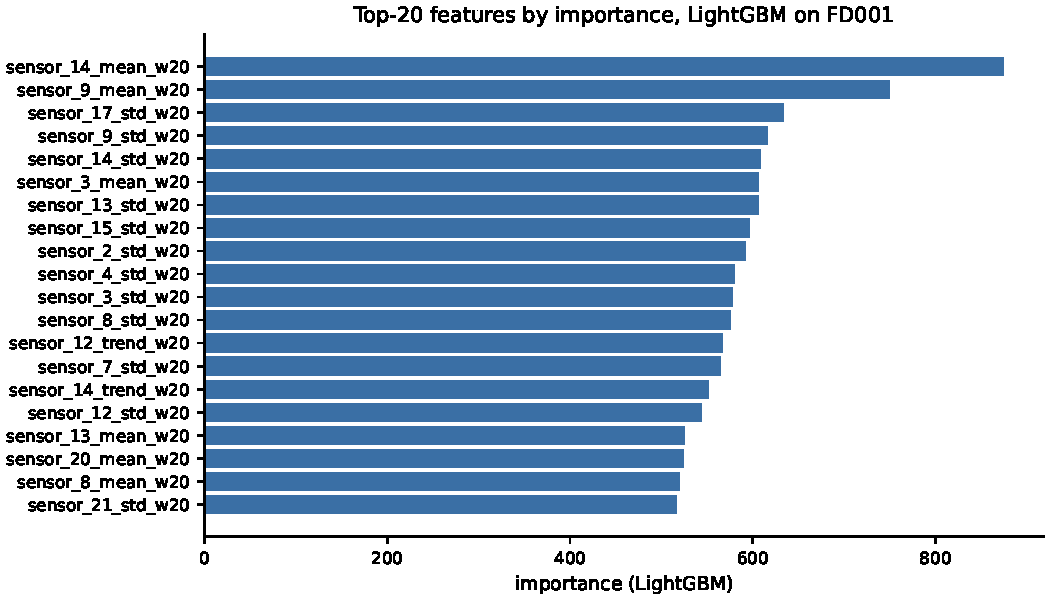
\includegraphics[width=0.80\linewidth]{fig_feature_importance.pdf}
\caption{Top-20 features by importance for the LightGBM model on FD001.
The ranking is dominated by rolling means, standard deviations, and
trends of sensors 14, 9, 17, 3, and 13, computed over the longer
($w = 20$) window.}
\label{fig:feature-importance}
\end{figure}

\subsection{A leakage trap worth documenting}\label{sec:leakage}
Our first tree model showed RMSE = 84.5 on FD001 --- worse than the
mean predictor (41.9) --- while ridge regression on the same features
gave a respectable 17.8. The disparity was suspicious enough to chase
down.

The culprit was a single feature we had added because it looked
``obviously useful'':
\begin{lstlisting}[language=Python]
df["cycle_norm"] = df.groupby("unit")["cycle"]\
                      .transform(lambda c: c / c.max())
\end{lstlisting}
On the training set every engine runs to failure, so
\verb|cycle_norm == 1.0| is perfectly correlated with
$\mathrm{RUL} = 0$. A boosted tree is a near-optimal learner of such
piecewise constant relationships and quickly latches on: ``if
\verb|cycle_norm| is close to 1 then predict $\mathrm{RUL} \approx 0$''.

In the test set, however, every engine is truncated \emph{before}
failure. The last recorded cycle in the test set still has
\verb|cycle_norm == 1.0|, but the true RUL at that point ranges from
7 to 145 cycles. The model, applied to that test set, confidently
predicts near-zero RUL for every healthy engine, and RMSE explodes.
Ridge regression escaped the trap because it found this feature only
weakly (linearly) correlated with the dozens of other features and gave
it modest weight; trees were perfectly suited to over-fit it.

The fix is one line:
\begin{lstlisting}[language=Python]
# Do NOT add cycle_norm: it leaks in training but not in test
\end{lstlisting}
After which RandomForest moved from RMSE~84.5 to~17.1, XGBoost from~69
to~15.7, and LightGBM from~76 to~15.9 on FD001.

\paragraph{Lesson.} In supervised prognostics with run-to-failure
training data and right-censored test data, any feature whose
\emph{denominator} comes from the training trajectory's length is
suspect. The bug would not have been caught by any train/validation
split that respected engine boundaries within the training set (because
training engines all run to failure), only by validating against
right-censored hold-out data. For industrial deployments this argues
strongly for keeping a small set of \emph{truncated} validation
trajectories aside, even when full-life data are available.

% ----------------------------------------------------------------------
\section{Deployment prototype}\label{sec:deployment}
% ----------------------------------------------------------------------
\subsection{REST API}
The trained LightGBM model is served behind a small Flask
\citep{ronacher2010flask} REST endpoint
(\verb|src/api.py| in the repository). The API accepts JSON of the form
\begin{lstlisting}[language={}]
{ "cycles": [[op1, op2, op3, s1, ..., s21],   // cycle 1
              [op1, op2, op3, s1, ..., s21],   // cycle 2
              ...                              // in chronological order
            ] }
\end{lstlisting}
and returns
\begin{lstlisting}[language={}]
{ "model": "LightGBM-FD001",
  "subset": "FD001",
  "n_cycles_received": 31,
  "predicted_RUL_cycles": 123.47,
  "warning_level": "OK",
  "recommended_action":
       "Continue normal operation. Re-evaluate after next cycle." }
\end{lstlisting}

The mapping from numerical RUL to maintenance action is intentionally
coarse:
\begin{center}
\small
\begin{tabular}{l l l}
\toprule
Predicted RUL & Warning level & Recommended action \\
\midrule
$> 80$ cycles & OK               & Continue normal operation. \\
$31$--$80$    & WATCH            & Add to elevated-attention list; review weekly. \\
$11$--$30$    & PLAN\_MAINTENANCE & Schedule maintenance within 10 cycles. \\
$\le 10$      & CRITICAL         & Bring asset offline at next opportunity. \\
\bottomrule
\end{tabular}
\end{center}
The exact thresholds would be tuned by the asset owner against the
PHM08-style cost ratios they care about; we ship sensible defaults.

\subsection{Dashboard}
A small Streamlit \citep{streamlit} dashboard
(\verb|src/dashboard.py|) lets an engineer pick one of the held-out
test engines, see its sensor traces and the model's prediction, and
read the recommended action. Figure~\ref{fig:dashboard} shows a static
mock-up rendered for FD001 engine~90, an engine whose true RUL is~28
cycles --- the model correctly predicts 26.7 cycles and surfaces the
\textsc{plan\_maintenance} recommendation.

\begin{figure}[t]
\centering
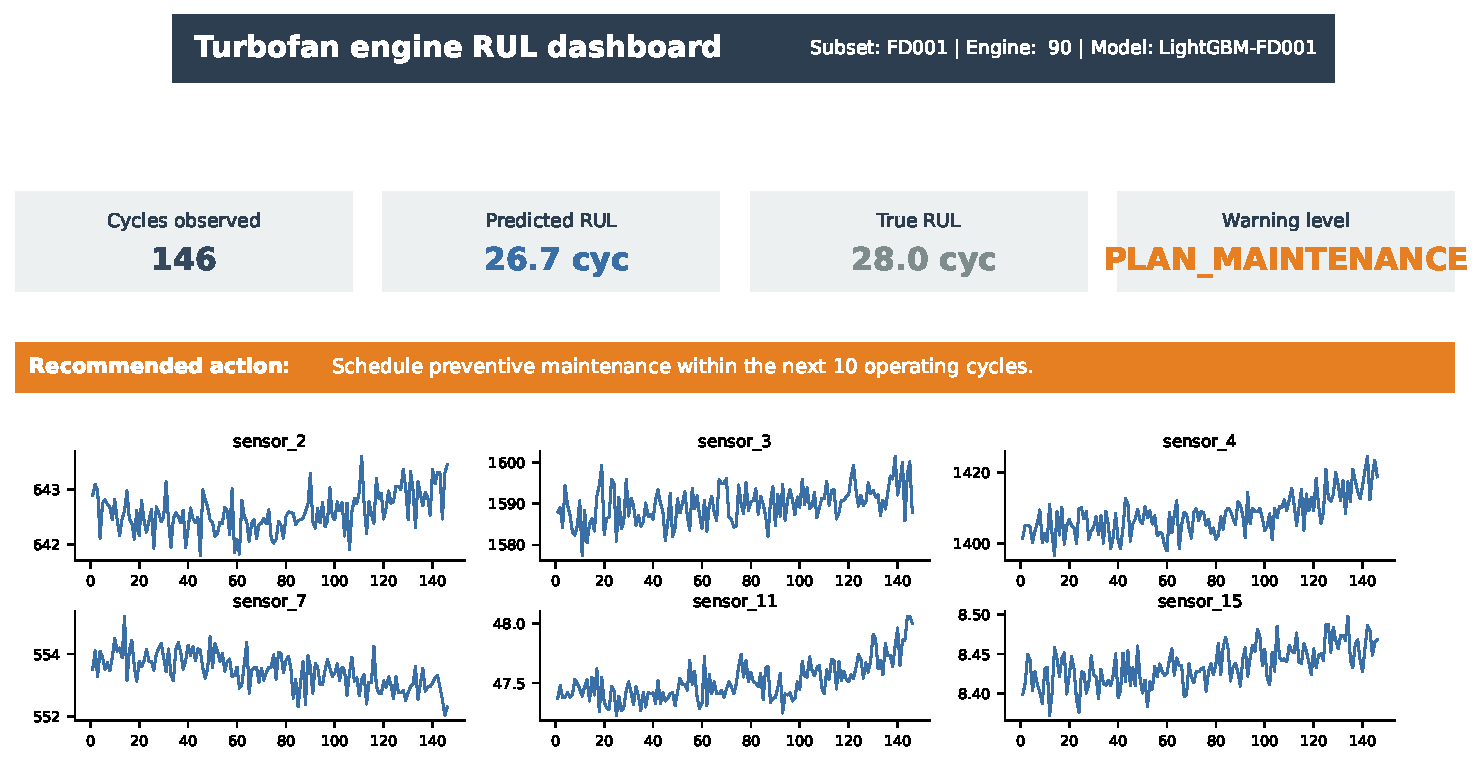
\includegraphics[width=0.95\linewidth]{fig_dashboard_mockup.pdf}
\caption{Static mock-up of the deployment dashboard for FD001
engine~90 (true RUL = 28). The model correctly recommends maintenance.
A real Streamlit screenshot would show the same layout in a web
browser; we render the mock-up with matplotlib because the testing
environment lacks a display server.}
\label{fig:dashboard}
\end{figure}

% ----------------------------------------------------------------------
\section{Limitations and what changes for SPM data}\label{sec:limitations}
% ----------------------------------------------------------------------
\paragraph{Simulation vs.\ real data.} CMAPSS data are generated by a
physics-based simulator, not collected on actual flying engines. The
noise model is therefore idealised, sensor faults are absent, missing
data are absent, and time stamps are perfectly synchronised across
channels. Real industrial monitoring data --- the kind originally
intended for this project --- will require an additional layer of
preprocessing for outlier detection, multi-rate sensor alignment, and
gap filling.

\paragraph{Vibration / frequency-domain features.} The CMAPSS sensor
suite is dominated by slowly-varying thermodynamic quantities
(temperatures, pressures, fan speeds). The proprietary data referenced
in the project plan would instead have been dominated by high-frequency
vibration signals already pre-processed via Fourier or envelope
transforms. The modelling backbone (regime-aware standardisation,
rolling features, LSTM) ports across unchanged, but the feature-extraction
stage would gain a dedicated spectral block: band-pass energy ratios
around bearing characteristic frequencies, kurtosis and crest factor of
the envelope spectrum, and so on \citep{randall2011vibration}.

\paragraph{Single fault mode per asset.} Even FD003/FD004 have only two
distinct fault modes. Real fleets present a longer tail of failure
modes (seal wear, blade-tip rub, bearing race spalling, lubrication
loss) each with its own degradation signature; a deployment-grade
system would need either a per-mode model or, more elegantly, a
multi-task model that predicts both the failure mode and the time to
failure.

\paragraph{Cost-sensitive thresholds.} The 80 / 30 / 10-cycle
thresholds in the deployment prototype are placeholders. A real
deployment should optimise them against the asset owner's actual cost
of unplanned downtime vs.\ scheduled inspection, ideally by running the
PHM08 score with an asymmetry coefficient tuned to that ratio.

\paragraph{Calibrated uncertainty.} The current model produces a point
estimate of RUL. For maintenance decisions one really wants a
\emph{predictive distribution} so that the recommendation can be tied
to a confidence interval (``95\% chance RUL $\le 30$'') rather than a
single number. Quantile regression \citep{koenker2005quantile} or
ensemble / Monte-Carlo dropout approaches \citep{gal2016dropout} are
the natural extensions.

% ----------------------------------------------------------------------
\section{Conclusion}\label{sec:conclusion}
% ----------------------------------------------------------------------
We built a complete, reproducible predictive-maintenance pipeline on
the publicly released NASA CMAPSS dataset: regime detection,
regime-aware standardisation, rolling-statistic features, a
piecewise-linear RUL target, five classical baselines, a PyTorch LSTM,
and a small Flask / Streamlit deployment prototype that translates
numerical RUL into categorical maintenance actions. Best test-set RMSE
is in the 14.5--15.5 range on every subset, competitive with published
benchmarks. The single most useful artefact to come out of the project
was probably a debugged failure mode: a tempting but leaky
\verb|cycle_norm| feature that inflated tree-model RMSE by a factor of
five and would not have been caught by a naive train/validation split.
We have argued that any deployment built on run-to-failure training
data should keep a small set of right-censored validation engines on
hand to catch this class of bug.

% ----------------------------------------------------------------------
\section*{Acknowledgements}
% ----------------------------------------------------------------------
The author thanks Prof.~Serdar Kadioglu for proposing and advising the
independent study, and the NASA Ames Prognostics Center of Excellence
for releasing the CMAPSS dataset under terms that permit academic
reuse. The dataset is acknowledged per the request of its custodians:
``A.~Saxena and K.~Goebel (2008). `Turbofan Engine Degradation
Simulation Data Set', NASA Prognostics Data Repository, NASA Ames
Research Center, Moffett Field, CA''.

% ----------------------------------------------------------------------
% References
% ----------------------------------------------------------------------
\bibliographystyle{plainnat}
\bibliography{refs}

\appendix
\section{Reproducibility}
\label{app:reproducibility}
All experiments were run on CPU (no GPU available in the test
environment), Python 3.12, in a Linux container. Key library versions:
\texttt{numpy 2.4}, \texttt{pandas 3.0}, \texttt{scikit-learn 1.8},
\texttt{xgboost 3.2}, \texttt{lightgbm 4.6}, \texttt{pytorch 2.12},
\texttt{scipy 1.17}. All random seeds set to~0. End-to-end wall-clock
on a single CPU container:
\begin{itemize}[leftmargin=*, itemsep=2pt, topsep=2pt]
\item Data download + parsing: $\le 10$~s
\item Exploratory analysis + figures: $\approx 30$~s
\item All tabular baselines on all four subsets: $\approx 4$~min
\item LSTM on FD001: $\approx 3$~min (24 epochs, early-stopped)
\item LSTM on FD002: $\approx 4$~min (12 epochs)
\item LSTM on FD003: $\approx 3$~min (25 epochs)
\item LSTM on FD004: $\approx 4.5$~min (10 epochs)
\end{itemize}
A modern GPU would reduce the LSTM training time by roughly an order of
magnitude; we did not need it to complete the study.

\section{Repository contents}
The code repository ships with the following deliverables, all
referenced from the \texttt{README.md}:
\verb|src/data_loader.py|, \verb|src/features.py|, \verb|src/eda.py|,
\verb|src/baselines.py|, \verb|src/lstm_model.py|,
\verb|src/result_figures.py|, \verb|src/api.py|,
\verb|src/dashboard.py|, \verb|src/dashboard_mockup.py|,
and the trained model files
\verb|models/lightgbm_FD001.joblib|,
\verb|models/xgboost_FD001.joblib|, \verb|models/xgboost_FD003.joblib|,
\verb|models/lstm_FD001.pt| through \verb|models/lstm_FD004.pt|.

\end{document}
